\documentclass[11pt]{report}

\usepackage{algorithmic}
\usepackage{algorithm}

% Set packages to be used (most should be included in your LaTeX installation; the rest are locally defined)
\usepackage{amsmath,amsfonts,amsthm,../styles/commands,graphicx,../styles/project}
% amsmath      : Provides enhanced functionality for mathematical formulas
%                ftp://ftp.ams.org/ams/doc/amsmath/amsldoc.pdf
% amsfonts     : Provides additional mathematical fonts
%                ftp://ftp.ams.org/pub/tex/doc/amsfonts/amsfndoc.pdf
% amsthm       : Provides enhanced commands for theorem-like environments
%                ftp://ftp.ams.org/ams/doc/amscls/amsthdoc.pdf
% commands     : Provides short-cut commands (locally defined)
% graphicx     : Provides enhanced support for graphics
%                http://en.wikibooks.org/wiki/LaTeX/Importing_Graphics#The_graphicx_package
% project      : Provides project format (locally defined)
% Other packages you may want to consider:
% amssymb, hyperref, longtable, natbib, rotating

\begin{document}

\title {A survey on some nonlinear programming algorithms}
\author{Xi He}

\preface
\chapter{Introduction}

This project concerns the practical implementation of several classical optimization algorithms in the context of unconstrained nonlinear problems. By choosing proper parameter set and delicate implementation, we intend to achieve economy of computation or the solution of such problems. With respect to several test problems, we compare the various performance of each algorithms with different parameters setup. It also might be a reasonable instruction on deciding which algorithm should be applied when faced a new problem.

At the first part of this project, we study several algorithms on solving unconstrained nonlinear optimization problems, such as steepest descent method, newton method and BFGS method with two kinds of linear search strategy: backtrack line search method and wolfe line search method. Trust region method is also argued with two similar approaches to solve trust region subproblem: conjugate gradient method and conjugate gradient method with SR1 Hessian matrix update method\footnote{Most of figures and algorithms pseudocode come from \cite{NoceWrig06}.}. Throughout the introduction of each algorithm, we also list convergence and complexity issues, however, one should note that we state some correct conclusions without rigorous proof.

In the latter part of this project, some detailed implementation concerns are discussed with respect to different problems and algorithms, including practical parameter set choosing, tricks on attaining economy computation and also some difficulties with respect to implementation. Results on numerical experiment are shown to clearly compare the performance of each algorithm with different parameters on each problem. Also, some analysis of the numerical result are presented.

The structure of this project report is as follows. Chapter 2 includes relevant background on unconstrained optimization problems which forms the basis of the discussions in later chapters. In Chapter 3, after showing the very basic two descent directions we used in implementation, we discuss two kinds of linear search strategy. And then we present two kinds of quasi-newton method and show the global convergence results when applying the two line search method mentioned before. We introduce in Chapter 4 about trust region algorithms and conjugate gradient method with is proposed by solving the trust region subproblems. SR1 update which is stated in Chapter 3 will be reconsidered as a approach to solving trust region subproblem when combining with conjugate gradient method. Finally, in Chapter 5, we present, analyze and provide numerical results with respect to the algorithms we discuss in above chapters on some test problems. Brief summary of this project and some general conclusion will be stated in the Chapter 6. 

In this report, we use the following notation. Let $f(x)$ be original nonlinear, smooth and differentiable objective function we want to minimize and $x$ be decision variables. We also denote gradient function of $f(x)$ by $g(x)=\nabla f(x)$ and denote $H(x)=\nabla^2 f(x)$ and $B(x)$ by the Hessian and approximation Hessian matrix of $f(x)$ at point $x$. With respect to algorithms, we use $d(x)$ to be an acceptable descent directions at point $x$ and $\alpha(x)$ to be an acceptable step-size along $d(x)$. At the last, $H\succ(\succeq) 0$ represents that the matrix is (semi) positive definite. 

\chapter{Fundamentals of Unconstrained Optimization}
We frame this report in the context of the unconstrained optimization problem
\begin{equation}
    \min_x \quad f(x),
\end{equation}

where $x\in \R^n$ is a real vector with $n\geq 1$ components $f:\R^n\rightarrow \R$ is a smooth function.

Generally, we intend to find out a global minimizer of $f$, a point where the function attains its least value in whole space. We state a formal definition as
\begin{definition}
    A point $x^*$ is a global minimizer if $f(x^*)\leq f(x)$ for all $x$.
\end{definition}

Note that it can be very difficult to find the global minimizer, since our knowledge of $f$ is usually only local. Actually, most algorithms are able to find only a local minimizer, a point that achieves the smallest value of $f$ in its neighborhood.
\begin{definition}
    A point $x^*$ is a local minimizer if there is a neighborhood $\Ncal$ of $x^*$ such that $f(x^*)\leq f(x)$ for $x\in \Ncal$.
\end{definition}

As it is shown in Figure \ref{fig:global_min}, in general case, a function $f$ may have a lot of local minimizers but just one global minimizer. Most algorithms is sensitive on the initial point we chose, which means, by choosing different initial point to run those algorithms, we may get different local minimizer.

\begin{figure}[H]
    \centering
    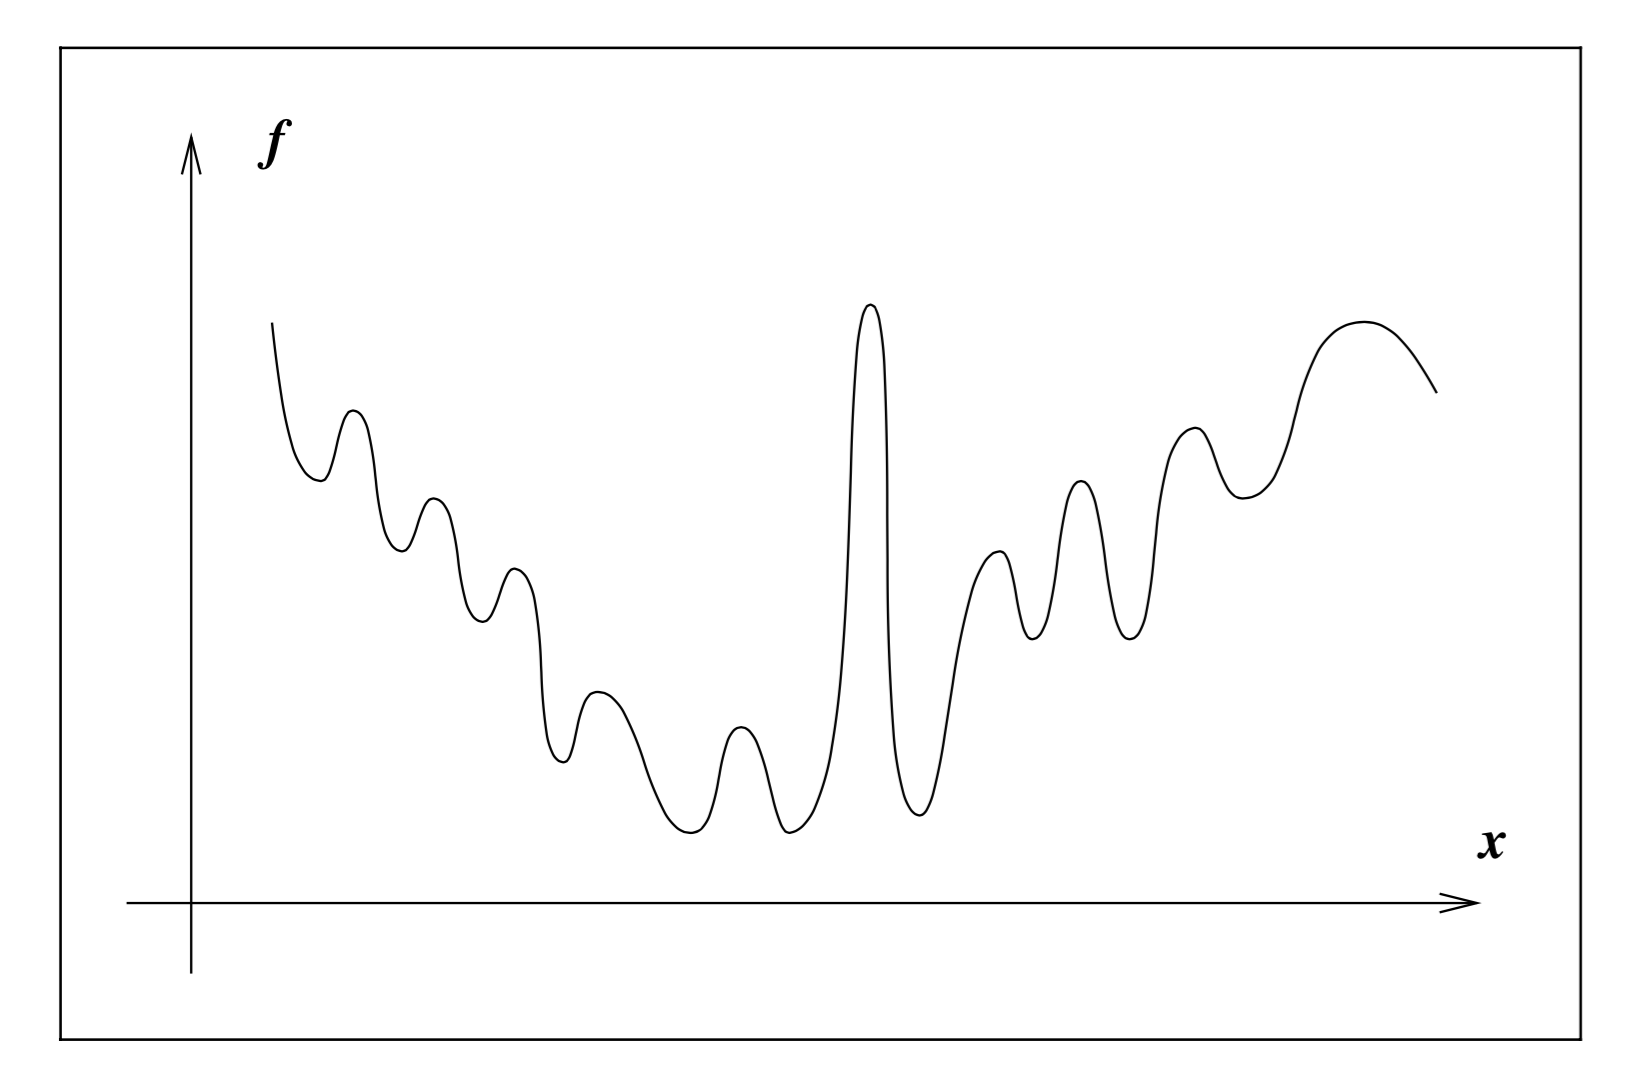
\includegraphics[width=0.95\textwidth]{../images/global_min}
    \caption{Global minimum and Local minimum}
    \label{fig:global_min}
\end{figure}

A special case we should concern is that of convex functions, every local minimizer is also a global minimizer. We state formal definition of convex as following
\begin{definition}
    A function $f: \R^n \rightarrow \R$ is convex if for all $\{x_1,x_2\}\in \R^n$ and $\alpha\in [0,1]$ we have
    \begin{equation}
        f(\alpha x_1 +(1- \alpha)x_2)\leq \alpha f(x_1) +(1- \alpha)f(x_2).
    \end{equation}
\end{definition}

Therefore, to solve a unconstrained optimization with respect to a convex objective function, we have conclusion that
\begin{theorem}
When $f$ is convex, any local minimizer $x^*$ is a global minimizer of $f$. If in addition $f$ is differentiable, then any stationary point $x^*$ is a global minimizer of $f$.
\end{theorem}

When turns to general case, i.e., objective function is not assuming to be convex but still smooth, we have following efficient and practical ways to identify local minima. To do it, we need have knowledge of the gradient $g(x^*)$ and the Hessian $H(x^*)$ of function $f$ at point $x^*$.
\begin{theorem}(First-Order Necessary Conditions)\label{thm:first_order}
    If $x^*$ is a local minimizer and $f$ is continuously differentiable in an open neighborhood of $x^*$, then $g(x^*)=0$.
\end{theorem}

We call $x^*$ a stationary point if $g(x^*)=0$. According to Theorem \ref{thm:first_order}, any local minimizer must be a stationary point. When consider Hessian matrix, we have the following conditions
\begin{theorem}(Second-Order Necessary Conditions)
If $x^*$ is a local minimizer of $f$ and $H$ is continuous in an open neighborhood of $x^*$, then $g(x^*) = 0$ and $H(x^*)$ is positive semidefinite.
\end{theorem}

Now, we state sufficient conditions, which are conditions on the derivatives of $f$ at the point $x^*$ that guarantee that $x^*$ is a local minimizer.
\begin{theorem}(Second-Order Sufficient Conditions)
Suppose that $H$ is continuous in an open neighborhood of $x^*$ and that $g(x^*) = 0$ and $H(x^*)$ is positive definite. Then $x^*$ is a strict local minimizer of $f$.  
\end{theorem}

\chapter{Algorithm Descriptions I: Flexible Step Method}\label{chp: flexible}
In flexible step method, general framework of algorithms is as following
\begin{algorithm}[H]
\caption{General Algorithm of Flexible Step Method}
\label{alg:General Flexible}
\begin{algorithmic}[1]
\REQUIRE Initial point $x_0$ and $k:=0$.
\REPEAT 
    \STATE Derive descent direction $d_k$ satisfying $g(x_k)^Td_k<0$
    \STATE Compute step-size $\alpha_k$ alone descent direction $d_k$ by line search method
    \STATE Update $x_{k+1} = x_k + \alpha_k d_k$, set $k = k + 1$
\UNTIL Termination condition satisfied.
\end{algorithmic}
\end{algorithm}

\section{Steepest Descent and Newton method}

Steepest descent direction and newton descent direction are two natural ways to get descent direction. In terms of steepest descent direction, due to $\norm{g(x)} >0$ when $x$ is not a stationary point, we can simply choose 
\begin{equation}
    d = -g(x),
\end{equation}

where we have $g(x)^Td = -\norm{g(x)}^2 <0$.

For newton descent method, first we note that if $H(x)$ is a positive definite matrix, we have $H(x)^{-1}$ is positive definite and furthermore $d^TH(x)^{-1}d >0$, whenever $d\neq 0$. By considering that since $g(x)\neq 0$ when $x$ is not a stationary point, we have 
\begin{equation}
    g(x)^TH(x)^{-1}g(x) >0,
\end{equation}

therefore, we can select 
\begin{equation}\label{eq: newton direction}
    d = -H(x)^{-1}g(x) 
\end{equation}

to be one possible descent direction. 

Besides, when $H(x)$ is not positive definite, we can perturb it to be positive definite by add positive number to its diagonal. Actually, we use the following procedure to implement this perturbation.
\begin{algorithm}[H]
\caption{Perturbation for non-positive definite matrix}
\label{alg:Perturbation for non-positive definite matrix}
\begin{algorithmic}[1]
\REQUIRE A non-positive definite matrix $P$ and a same-size identity matrix $I$
%\STATE Set $\eta = 10^{-4}$
\IF {$\min\mbox{eig}(P)<0.1$}
    \STATE $P = P + (1-\min\mbox{eig}(P)) I$
%    \STATE $\eta = 10\eta$
\ENDIF
\STATE Output a positive definite matrix $P$
\end{algorithmic}
\end{algorithm}

Note that by using this approach, we guarantee the perturbed matrix $P$ to be positive definite and its minimal eigenvalue is at least greater than $0.9$, which suppose to be well-defined matrix when solving the linear system \eqref{eq: newton direction}.

After we pick up a descent direction, we need find a proper step-size, which is what we called line search method in the next section.

\section{Line Search Methods}\label{sec:Line_search}

Always, step-size are chosen to give a sufficient reduction of $f$, but at the same time, we prefer to spend less time to choose a proper step-size. At current point $x_k$ with a descent direction $d_k$, we let
\begin{equation}
    \phi(\alpha) = f(x_k + \alpha d_k), \alpha>0, 
\end{equation}

we may say the ideal choice is to find a global minimizer $\alpha^*$ of the one-dimensional function $\phi(\alpha)$. However, it is too costly to find the global minimizer. Therefore, we apply some more practical strategies that calculating step in an inexact approach. In this project, we discuss two kinds of line search method as following.

\subsection{Wolfe Conditions} % (fold)
\label{ssub:wolfe_conditions}

It contain two parts when find a proper step-size by wolfe conditions. Firstly, we should choose a step-size that provide sufficient reduction. We use the following condition to guarantee it
\begin{equation}\label{eq: Wolfe_suff_decrease}
    f(x_k+\alpha d_k) \leq f(x_k) + c_1 \alpha \nabla f_k^Td_k,
\end{equation}

which $c_1\in (0,1)$ is a parameter. By noting that $ \nabla f_k^Td_k<0$ since $d_k$ is a descent direction, we say that \eqref{eq: Wolfe_suff_decrease} is sufficient decrease condition. We show geometry explanation in Figure~\ref{fig: Wolfe_suff_decrease}.

\begin{figure}[H]
    \centering
    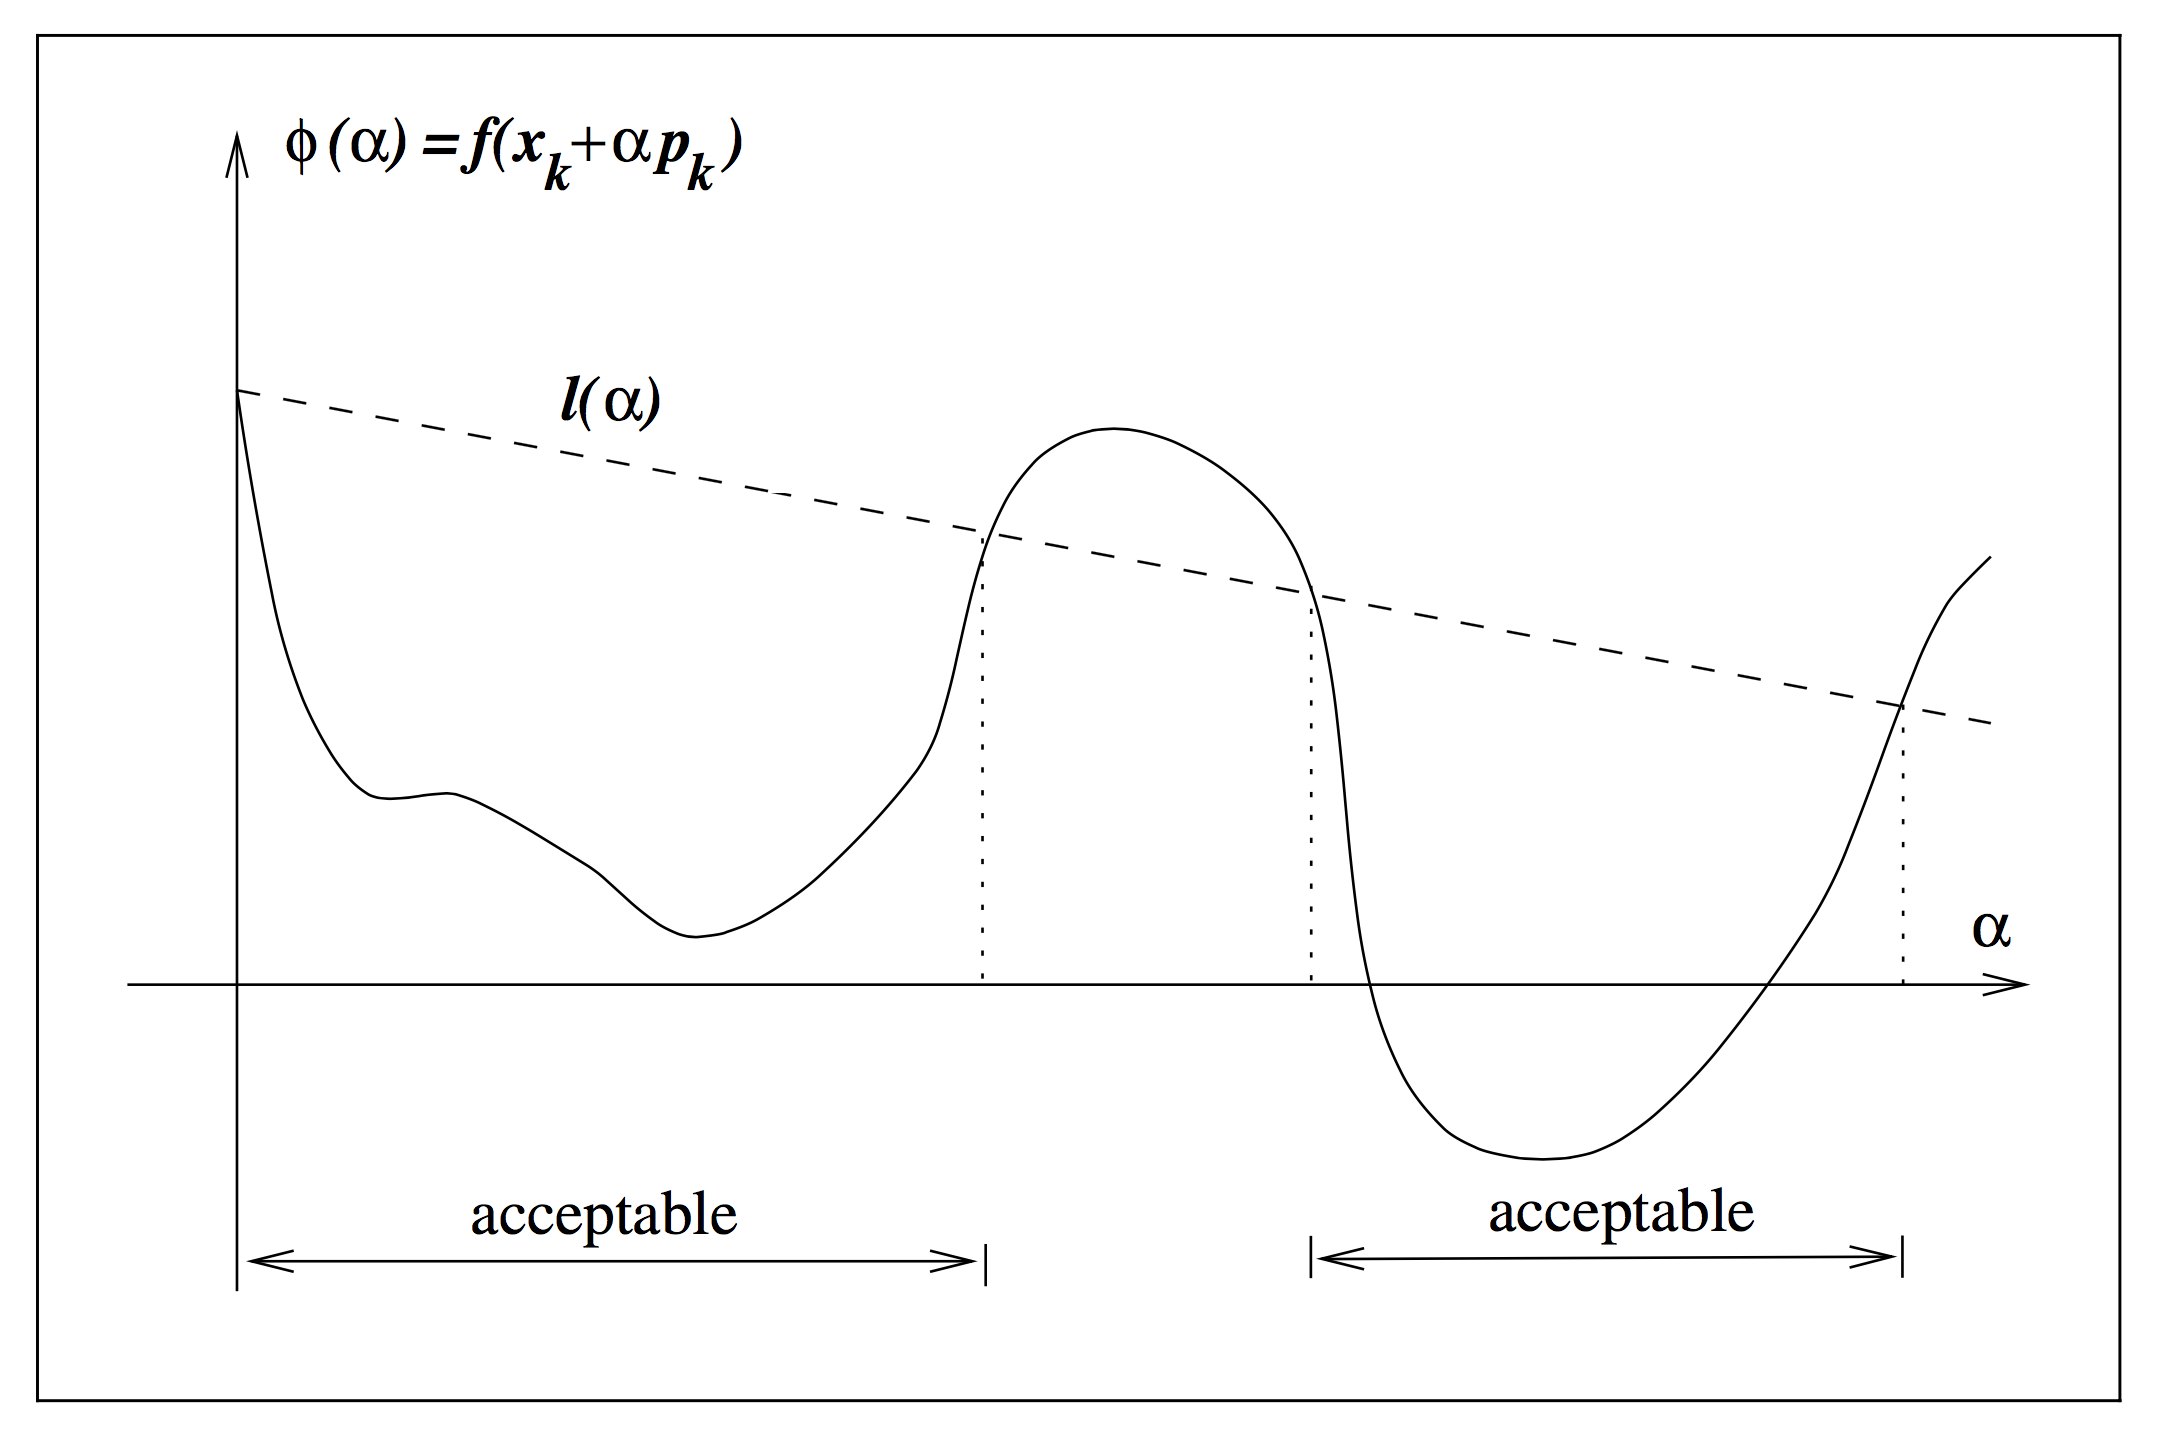
\includegraphics[width=0.75\textwidth]{../images/wolfe1} 
    \caption{Sufficient decrease condition}
    \label{fig: Wolfe_suff_decrease}
\end{figure}

Except this condition, we make other condition called curvature condition to get rid of unacceptably short steps
\begin{equation}\label{eq:wolfe_curvature}
    \nabla f(x_k+\alpha_k p_k)^T \geq c_2 \nabla f_k^Tp_k,
 \end{equation}

 where $c_2\in (c_1,1)$ is another parameter. Geometry illustration is shown in Figure~\ref{fig:Wolfe_curvature}.
\begin{figure}[H]
    \centering
    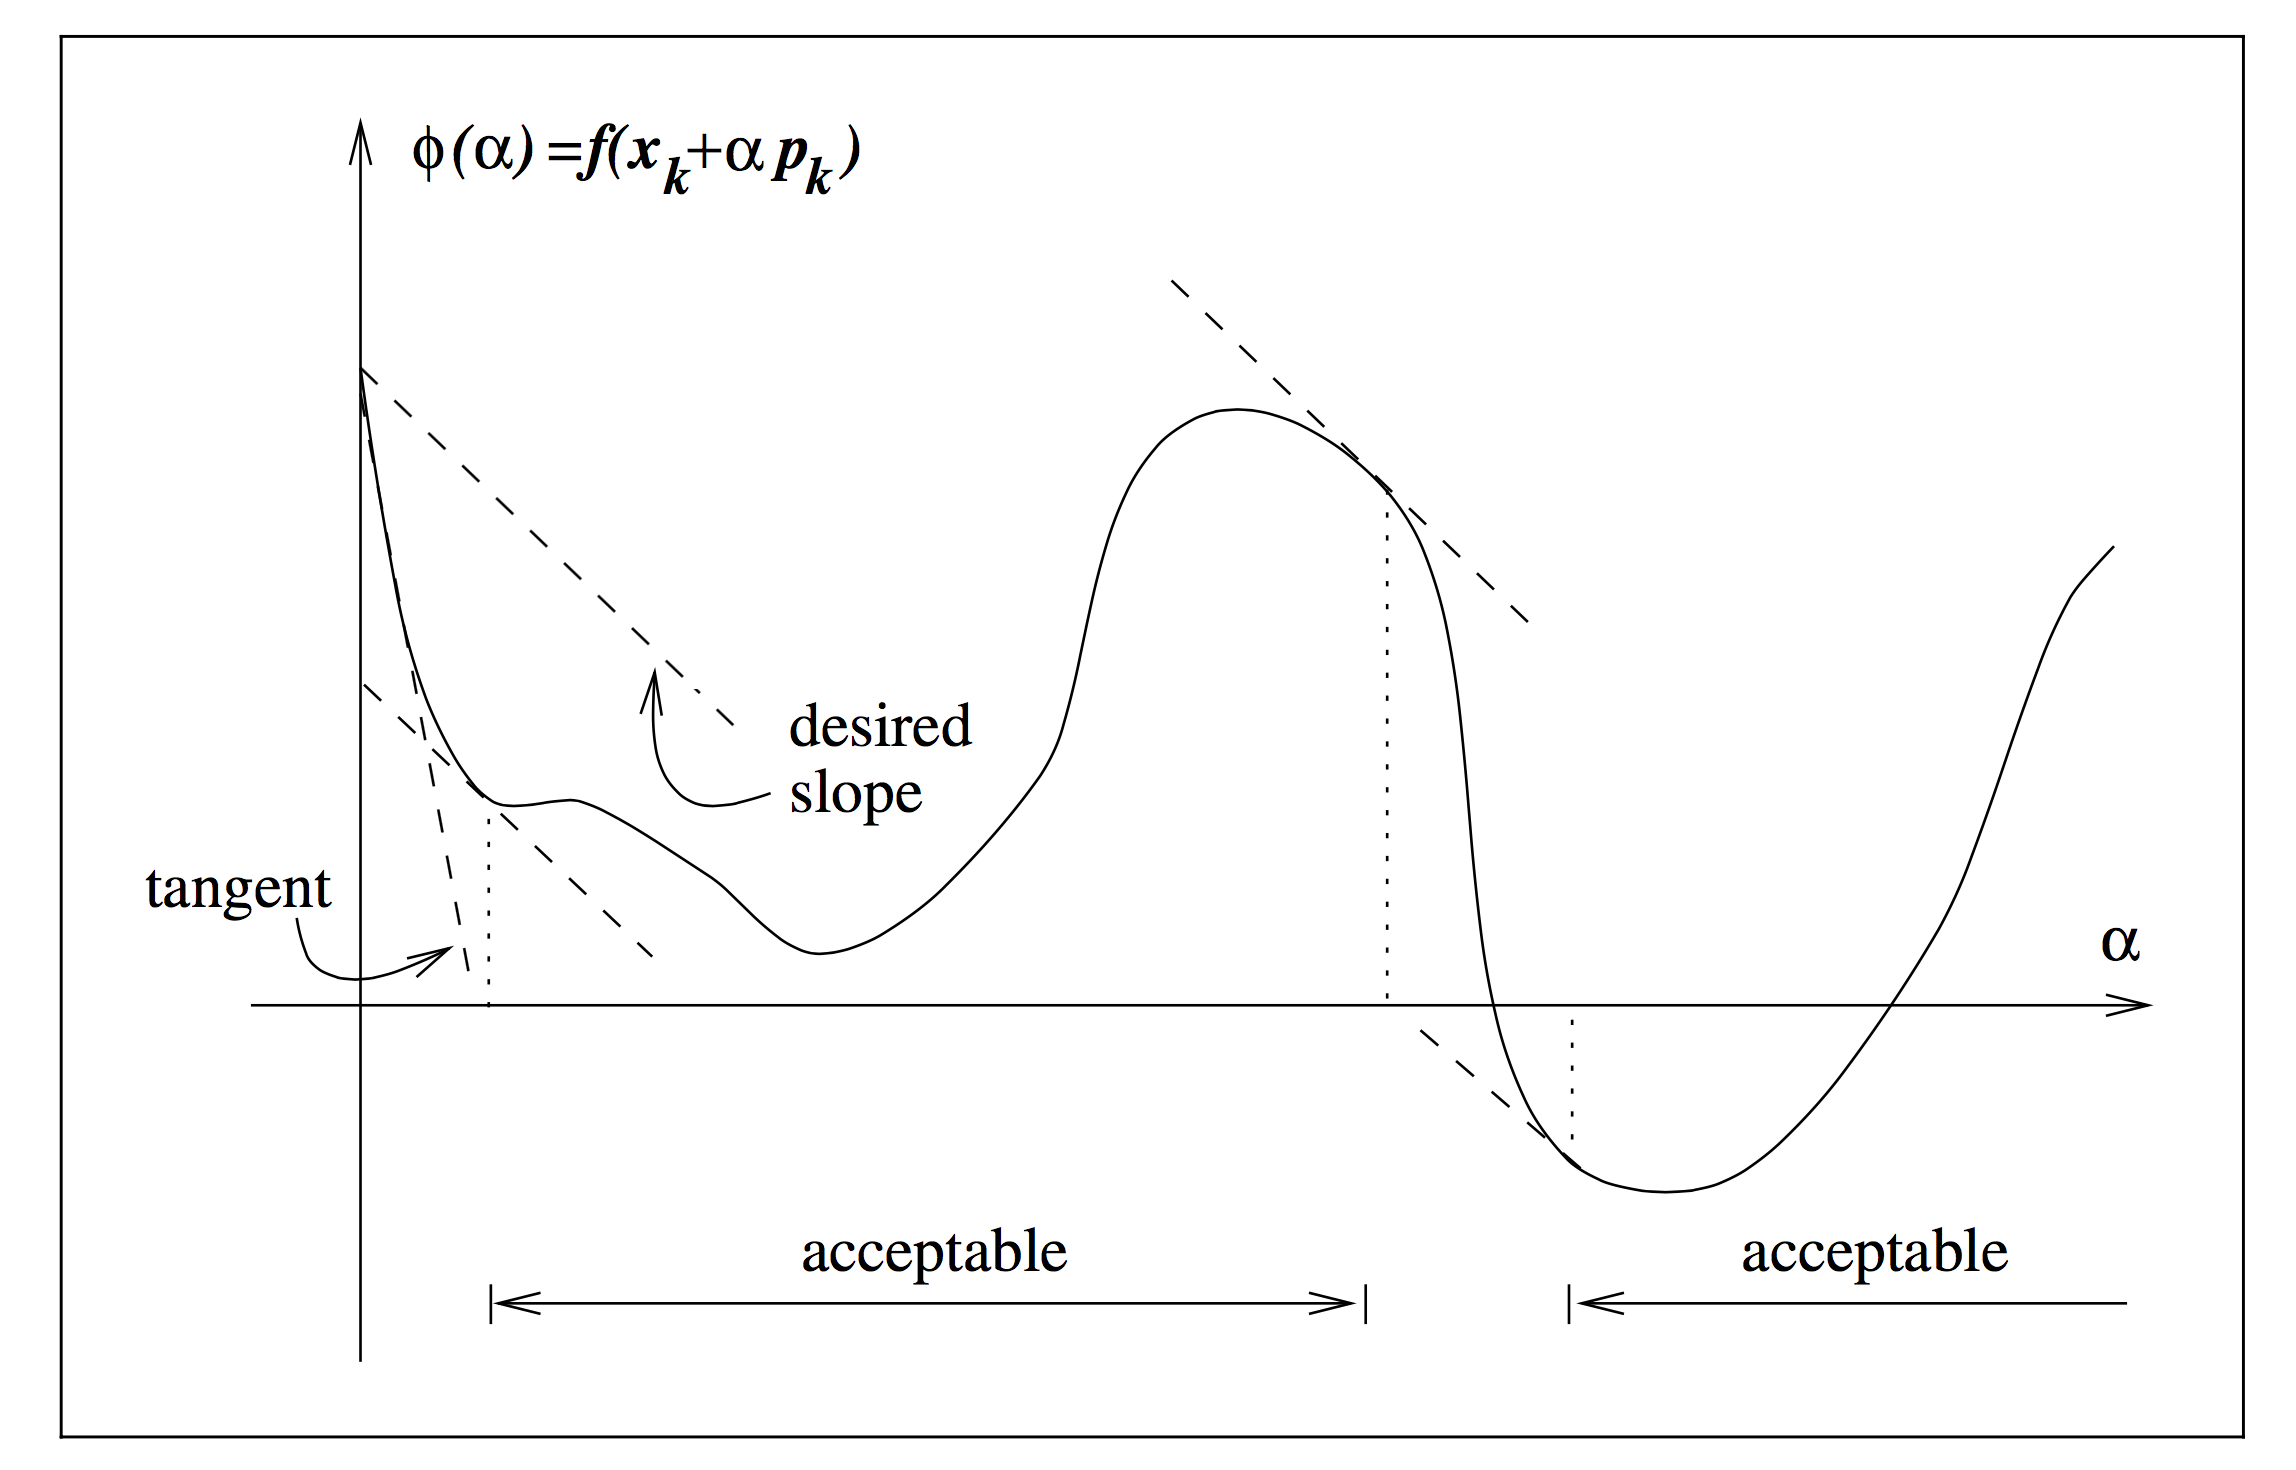
\includegraphics[width=0.75\textwidth]{../images/wolfe2}
    \caption{Wolfe curvature condition}
    \label{fig:Wolfe_curvature}
\end{figure}

Practically, we implement wolfe condition as following
\begin{algorithm}[H]
\caption{Wolfe Conditions}
\label{alg:Wolfe Conditions}
\begin{algorithmic}[1]
\REQUIRE Initial step-size $\alpha_0 >0$, $\alpha_1 >0$ and $\alpha_{\max}$. Set $i:= 1$. 
\STATE $\alpha = \bar{\alpha}$
\REPEAT
    \IF  {$\phi(\alpha_i) > \phi(0) + c_1 \alpha_i \phi'(0)$ or [$\phi(\alpha_i)\geq \phi(\alpha_{i-1}) \mbox{ and } i>1$]  }
    \STATE $\alpha_*  \leftarrow \mathbf{zoom}(\alpha_{i-1},\alpha_i)$ and stop;
    \ENDIF
    \IF {$|\phi'(\alpha_i)| \leq -c_2\phi'(0)$}
    \STATE set $\alpha_* \leftarrow a_i$ and stop;
    \ENDIF
    \IF {$\phi'(\alpha_i) \geq 0$}
    \STATE set $\alpha_* \leftarrow \mathbf{zoom}(\alpha_i,\alpha_{i-1})$ and stop;
    \ENDIF
    \STATE Choose $\alpha_{i+1} \in (\alpha_i,\alpha_{\max})$
    \STATE $i \leftarrow i+1$
\UNTIL{}
\STATE Terminate with $\alpha_k = \alpha$
\end{algorithmic}
\end{algorithm}

Here zoom function is proposed to find a proper step-size in an interval.
\begin{algorithm}[H]
\caption{Wolfe Conditions (zoom function)}
\label{alg:Wolfe Conditions zoom function}
\begin{algorithmic}[1]
\REQUIRE Initial step-size $\alpha_{low} >0$ and $\alpha_{high} >0$ 
\REPEAT
\STATE Choose $\alpha_j$ between $\alpha_{low}$ and $\alpha_{high}$.
    \IF  {$\phi(\alpha_j) > \phi(0) + c_1 \alpha_j \phi'(0)$ or $\phi(\alpha_j)\geq \phi(\alpha_{low})$}
    \STATE $\alpha_{high}\leftarrow \alpha_j$
    \ELSE
    \IF {$|\phi'(\alpha_j)| \leq -c_2\phi'(0)$}
    \STATE set $\alpha_* \leftarrow a_j$ and stop
    \ENDIF
    \IF {$\phi'(\alpha_i)(\alpha_{high}-\alpha_{low}) \geq 0$}
    \STATE set $\alpha_{high} \leftarrow \alpha_{low}$
    \ENDIF
    \STATE $\alpha_{low} \leftarrow \alpha_j$
    \ENDIF
\UNTIL{}
\end{algorithmic}
\end{algorithm}

% subsubsection wolfe_coniditions (end)

\subsection{Backtracking Line Search}
Another popular approach is to drop curvature condition \eqref{eq:wolfe_curvature} by appropriately choosing candidate step lengths, which we called backtracking strategy.
\begin{algorithm}[H]
\caption{Backtracking Line Search}
\label{alg:Backtracking Line Search}
\begin{algorithmic}[1]
\REQUIRE Initial step-size $\bar{\alpha} >0$ and shrinking parameter $\rho \in (0,1)$
\STATE $\alpha = \bar{\alpha}$
\REPEAT
    \STATE $\alpha = \rho \alpha$
\UNTIL{$f(x_k+ \alpha p_k) \leq f(x_k) + c \alpha \nabla f_k^Tp_k$}
\STATE Terminate with $\alpha_k = \alpha$
\end{algorithmic}
\end{algorithm}

Global convergence result for line search methods with respect to steepest descent method is proved under some mild assumption. 

\section{Quasi-newton method}\label{sec: Quasi-newton method}
Another approach to derive descent direction is to use Quasi-newton method, which only depends on only first derivatives. Actually, what we do in Quasi-newton method is to approximate Hessian matrix by first derivatives instead of computing accurate Hessian matrix directly, which is sometimes computational expensive.

In this project, we use BFGS method to update Hessian matrix with flexible step, which is one type of Quasi-newton method. 

Let $B_k$ be BFGS approximate Hessian matrix at point current point $x_k$. And then we can derive descent direction from
\begin{equation}\label{eq:BFGSupdate}
    B_kd_k = -\nabla f(x_k). 
\end{equation}

Furthermore, we have $x_{k+1} = x_k + a_kd_k$, where $a_k$ is a proper step-size derived from line search method in section \ref{sec:Line_search}. By defining
\begin{equation}
    s_k = x_{k+1} - x_k \mbox{~and~} y_k = \nabla f_{k+1} - \nabla f_k,
\end{equation}

we have 
\begin{equation}
    B_{k+1} = B_k -\frac{B_ks_ks_k^TB_k}{s_k^TB_ks_k}+\frac{y_ky_k^T}{y_k^Ts_k},
\end{equation}

where $-\frac{B_ks_ks_k^TB_k}{s_k^TB_ks_k}+\frac{y_ky_k^T}{y_k^Ts_k}$ is a rank two matrix which only depends on first derivatives. Notice that to derive descent direction by \eqref{eq:BFGSupdate}, we need guarantee $B_k$ to be positive definite, luckily, as long as $B_k\succ 0$  and the curvature condition
\begin{equation}
    s_k^Ty_k >0
\end{equation}

is satisfied, then we have $B_{k+1}$ is positive definite.

Practically, we use damped BFGS updating to overcome some shortage of BFGS updating, such as to avoid $y_k^Ts_k\approx 0$ or poorly conditioned Hessian approximation. We state damped BFGS updating as following
\begin{algorithm}[H]
\caption{Damped BFGS updating}
\label{alg:Damped BFGS updating}
\begin{algorithmic}[1]
\REQUIRE $H_k$, $s_k=x_{k+1}-x_k$ and $r_k = \nabla f(x_{k+1})-\nabla f(x_k)$ at current point $x_k$. A parameter $\theta$.
\STATE Compute
\begin{equation}
    \theta_k = \begin{cases}
        1, & \mbox{if~~} r_k^Ts_k \geq \theta s_k^TH_ks_k\\
        \frac{(1-\theta)s_k^TH_ks_k}{s_k^TH_ks_k-r_k^Ts_k}, &\mbox{otherwise}
    \end{cases}
\end{equation}
\STATE Set $y_k = \theta_k r_k + (1-\theta_k)H_ks_k$
\end{algorithmic}
\end{algorithm}

By this procedure, we guarantee that 
\begin{equation}
    y_k^Ts_k \geq \theta s_k^TH_ks_k >0,
\end{equation}

which leads to a well-defined BFGS updating.

It is proved that BFGS method with Wolfe line search is global convergent and shares a superlinear convergence rate. 

\chapter{Algorithm Descriptions II: Restricted Step Methods.}\label{chp: restricted}

In restricted step method, general framework of algorithms is as following
\begin{algorithm}[H]
\caption{General Algorithm of Restricted Step Method}
\label{alg:General Restricted}
\begin{algorithmic}[1]
\REQUIRE Initial point $x_0$ and $k:=0$.
\REPEAT 
    \STATE Generate a proper subproblem $G(d)$ at $x_k$
    \STATE Solve subproblem to derive descent direction $d_k$
    \STATE Update $x_{k+1} = x_k + d_k$, set $k = k + 1$
\UNTIL Termination condition satisfied.
\end{algorithmic}
\end{algorithm}

\section{Trust Region Method}
Instead of calculate step size at each iteration, trust region method is one other approach to solve nonlinear optimization problems. In a sense, trust region is a restricted step method as the direction and step size are uniquely decided at each iteration. The main idea of trust region method is to generate a subproblem on a neighborhood of current point $x_k$. Normally, we set the subproblem as
\begin{align}\label{eq: trust region subproblem}
\min_{d_k}\quad & m_k(d_k) := f(x_k) + \nabla f(x_k)^Td_k + \frac{1}{2}d_k^TH_kd_k\\
s.t. \quad & \norm{d_k} \leq \Delta_k.
\end{align}

Note that $m_k(d_k)$ is a approximate function of $f$ at point $x_k$ and with respect to $H_k$, we often set $H_k\succ 0$, but not necessarily, for example, we can choose $H_k$ to be the SR1 approximate Hessian matrix. 

Therefore, based on the framework \ref{alg:General Restricted}, we have the following algorithm
\begin{algorithm}[H]
\caption{Trust Region Method}
\label{alg:Trust Region Method}
\begin{algorithmic}[1]
\REQUIRE Current point $x_k$, trust region radius $\Delta_k$, subproblem $m_k(d_k)$ and two threshold $0<c_1 <c_2 <1$.
\REPEAT
\STATE Solve subproblem $m_k(d_k)$
\STATE Compute the ratio
\begin{equation}
    \rho_k(d_k) := \frac{f(x_k)-f(x_k+d_k)}{m_k(0)-m_k(d_k)}.
\end{equation}
\IF{$\rho_k(d_k) \geq c_2$}
\STATE Update $x_{k+1} = x_k + d_k$ and expand trust region $\Delta_{k+1} > \Delta_k$
\ELSE
\IF{$\rho_k(d_k) \in (c_1, c_2)$}
\STATE Update $x_{k+1} = x_k + d_k$ and keep trust region $\Delta_{k+1} = \Delta_k$
\ENDIF
\ELSE
\IF{$\rho_k(d_k) \leq c_1$}
\STATE Keep $x_{k+1} = x_k$ and shrink trust region $\Delta_{k+1} < \Delta_k$
\ENDIF
\ENDIF
\UNTIL{Meet termination condition}
\end{algorithmic}
\end{algorithm}

\section{Conjugate Gradient Method}
By deriving a set of $n$ vectors which is all conjugated for each other, we build a cheaper way to compute descent direction for quadratic problem
\begin{equation}
    \min_x \quad \phi(x) := \frac{1}{2}x^TAx - b^Tx.
\end{equation}

Actually, if we have a set of conjugated direction $\{p_0,\dots,p_{n-1}\}$, we can solve the problem in at most $n$ steps by repeating the following procedure
\begin{itemize}
    \item Compute the current residual
    \begin{equation}
        r_k = Ax_k - b
    \end{equation}
    \item Compute a steplength to minimize $\phi(x)$ along $x_k+\alpha p_k$
    \begin{equation}
        \alpha_k = -\frac{r_k^Tp_k}{p_k^TAp_k}
    \end{equation}
    \item Update $x_{k+1} = x_k +\alpha_k p_k$
\end{itemize}

Actually, by letting the first conjugated direction $p_0= -r_0$, we can derive others conjugated direction step by step by the following algorithm
\begin{algorithm}[H]
\caption{Conjugate Direction Method}
\label{alg:Conjugate Direction Method}
\begin{algorithmic}[1]
\REQUIRE Initial point $x_0$, set $r_0 = Ax_0-b$ and $p_0=-r_0$
\REPEAT
\STATE $\alpha_k = \frac{r_k^Tr_k}{p_k^TAp_k}$
\STATE $ x_{k+1} = x_k + \alpha_kp_k$
\STATE $ r_{k+1} = r_k + \alpha_kAp_k$
\STATE $ \beta_{k+1} = \frac{r_{k+1}^Tr_{k+1}}{r_k^Tr_k}$
\STATE $ p_{k+1} = -r_{k+1} + \beta_{k+1}p_k$
\UNTIL{Meet termination condition}
\end{algorithmic}
\end{algorithm}

\section{Trust Region Subproblem with CG Method}
Here we state a nice approach to solve the trust region subproblem \eqref{eq: trust region subproblem}. 
\begin{algorithm}[H]
\caption{Trust Region Subproblem with CG Method}
\label{alg:Trust Region Subproblem with CG Method}
\begin{algorithmic}[1]
\REQUIRE Initial point $x_0$, trust region radius $\Delta_k$ and we set $r_0 = Ax_0-b$ and $p_0=-r_0$
\REPEAT
\IF{$p_k^TAp_k<0$}
\STATE Set $\alpha_k$ to be a positive value such that $\norm{x_k+\alpha_kp_k}_2 = \Delta_k$
\STATE Update $x_{k+1} = x_k + \alpha_k p_k$ and stop
\ELSE
\STATE $\alpha_k = \frac{r_k^Tr_k}{p_k^TAp_k}$
\ENDIF
\IF{$\norm{x_k+\alpha_kp_k}_2 > \Delta_k$}
\STATE Set $\alpha_k$ to be a positive value such that $\norm{x_k+\alpha_kp_k}_2 = \Delta_k$
\STATE Update $x_{k+1} = x_k + \alpha_k p_k$ and stop
\ELSE
\STATE $x_{k+1} = x_k + \alpha_k p_k$ and $r_{k+1} = r_k + \alpha_kAp_k$
\ENDIF
\IF{$\norm{r_{k+1}}_2 \approx 0$}
\STATE Update $x_{k+1} = x_k + \alpha_k p_k$ and stop
\ELSE
\STATE $\beta_{k+1} =\frac{r_{k+1}^Tr_{k+1}}{r_k^Tr_k}$ and $ p_{k+1} = -r_{k+1} + \beta_{k+1}p_k$
\ENDIF
\UNTIL{Meet termination condition}
\end{algorithmic}
\end{algorithm}

Note that in this algorithm, $A$ can be chosen directly as Hessian matrix at current point $x_k$ or SR1 approximate Hessian matrix. With respect to SR1 update, which means to update $A(H_k)$ by the following formula
\begin{equation}
    H_{k+1} = H_k + \frac{(y_k-H_ks_k)(y_k-H_ks_k)^T}{(y_k-H_ks_k)^Ts_k},
\end{equation}

where $y_k$ and $s_k$ are defined same as BFGS method in Section \ref{sec: Quasi-newton method}, and $ \frac{(y_k-H_ks_k)(y_k-H_ks_k)^T}{(y_k-H_ks_k)^Ts_k}$ is a rank-one matrix.

Note that to make this update well-defined, we need the extra judgment that
\begin{equation}
    |(y_k-H_ks_k)^Ts_k| \geq c \norm{y_k-H_ks_k}\norm{s_k},
\end{equation}

where $c\in(0,1)$ is a user-specified constant. Also there is no guarantee that this update $H_{k+1}\succ 0$ even if $H_k\succ 0$.  However, it is not necessary to restrict $H_k$ to be positive definite, since the trust region subproblem are a constraint optimization problems.
\chapter{Numerical Results}

This chapter contains numerical results with respect to those algorithms we discussed in Chapter \ref{chp: flexible} and \ref{chp: restricted}. 

Note that all algorithms are implemented by Matlab under Intel Core $i5$ $2.6$ GHz processor and $8$ GB memory. Throughout this chapter, with respect to each algorithm, we use $Iter.$ to represent the total number of Iterations it takes to meet termination conditions. If the actual $Iter.$ is greater than defined $maxiter$, we mark $Iter.$ by a slash. $Cputime$ stands for total time of a algorithms spend to find the minimizer and when the corresponding $Iter.$ is marked as a slash, $Cputime$ means time cost up to $maxiter$ iteration. We denote $xNorm$ by the norm of difference between ending point of an algorithm and the accurate minimizer. $gNorm$ represents for the norm of gradient at the ending point.

We begin by providing some general comments that may be useful for achieve a economy computation. 

We set the default parameter value as following
\begin{table}[htpb]
    \caption{Default Parameter Set}
    \label{tab:default_para}
    \begin{center}
        \begin{tabular}{l|ccccc}
        \hline
        \hline
        \textbf{i} & \textbf{maxiter} & \textbf{opttol} & \textbf{(c1ls,c2ls)}& \textbf{(c1tr,c2tr)}\\
        \hline
             \textbf{value}& $1000$&$10^{-6}$ & $(10^{-4},0.9)$ &${(0.3,0.9)}$\\
        \hline
        \hline
        \textbf{i} & \textbf{cgopttol}& \textbf{cgmaxiter}& \textbf{sr1updatetol}& \textbf{bfgsupdatetol}& \textbf{initialradius} \\
        \hline
         \textbf{value}& $10^{-6}$& $50$ & $10^{-6}$ & $0.2$ &$0.25$\\
        \hline
        \hline
        \textbf{i} & \textbf{perturbHession}& \textbf{shrinkradius}& \textbf{expandradius}& \textbf{shrinkbacktrack}& \textbf{residuetol} \\
        \hline
         \textbf{value}& $10^{-4}$& $0.25$ & $2$ & $0.25$ &$10^{-6}$\\
        \hline
        \hline
        \textbf{i} & \textbf{wolfemax}& \textbf{posdeftol}& \textbf{mineigtol} \\
        \hline
         \textbf{value}& $10$& $0.1$ & $1.0$\\
        \hline
        \hline
        \end{tabular}
    \end{center}
\end{table}

By this default set, we state numerical results for all four test problems, respectively.

\textbf{(1) Rosenbrock }

Objective function: 
\begin{equation}
    f(x_1,x_2) = 100(x_2-x_1^2)^2+(1-x_1)^2.
\end{equation}

Accurate minimizer:
\begin{equation}
    (x_1,x_2) = (1,1).
\end{equation}

Numerical results with initial point $0\mathbf{e}$:
\begin{table}[H]
    \caption{Rosenbrock, with initial $0\mathbf{e}$}
    \label{tab:Rosenbrock_initial}
    \begin{center}
        \begin{tabular}{l|ccccccc}
\textbf{ROSENBROCK}&    gNorm       &   Iter.  &   Cputime   &   feval&geval&Hevel&Linsolved\\
\hline
steepestbacktrack   &   $1.000e-01 $&   $- $&   $0.3856  $&$6236 $&$1002 $&$0    $&$0    $       \\
steepestwolfe       &   $1.010e-01 $&   $- $&   $0.8075  $&$18629$&$2071 $&$0    $&$0    $       \\
newtonbacktrack     &   $7.406e-07 $&   $13   $&   $0.0544  $&$30   $&$14   $&$13   $&$13   $       \\
newtonwolfe         &   $3.652e-10 $&   $14   $&   $0.0500  $&$49   $&$19   $&$14   $&$14   $       \\
trustregioncg       &   $1.019e-06 $&   $54   $&   $0.0784  $&$55   $&$32   $&$32   $&$0    $       \\
sr1trustregioncg    &   $8.581e-07 $&   $68   $&   $0.0642  $&$69   $&$42   $&$0    $&$0    $       \\
bfgsbacktrack       &   $3.416e-08 $&   $23   $&   $0.0530  $&$55   $&$24   $&$0    $&$23   $       \\
bfgswolfe           &   $6.357e-07 $&   $21   $&   $0.0580  $&$76   $&$27   $&$0    $&$21   $       \\
     \end{tabular}
    \end{center}
\end{table}

Rosenbrock function is supposed to be create to illustrate the inefficiency of steepest descent method. Especially, when current point lies in some area nearby the optimal point $(1,1)$, the convergent rate decrease dramatically. By checking its contour, which we call banana shape, it shows that in such a long and narrow arrow, steepest descent direction are roughly orthogonal with each other. This fact lead to low convergence result. However, with respect to other algorithms, their performance are somehow similar.  They all lead to a minimizer in roughly same iterations.


\textbf{(2) Genhumps }

Objective function: 
\begin{equation}\label{genhumps}
    f(x) = \sum_{i=1}^4(\sin(2x_i)^2\sin(2x_{i+1})^2+0.05(x_i^2+x_{i+1}^2)).
\end{equation}

Accurate minimizer:
\begin{equation}
    x = 0\mathbf{e}  .
\end{equation}

Numerical results with initial point $\mathbf{e}$:
\begin{table}[H]
    \caption{Genhumps, with initial $\mathbf{e}$}
    \label{tab:Genhumps_initial}
    \begin{center}
        \begin{tabular}{l|ccccccc}
\textbf{GENHUMPS}&  gNorm       &   Iter.  &   Cputime   &   feval&geval&Hevel&Linsolved\\
\hline
steepestbacktrack   &   $3.589e-06 $&   $102  $&   $0.1166  $&$261  $&$103  $&$0    $&$0    $       \\
steepestwolfe       &   $3.884e-06 $&   $145  $&   $0.1051  $&$572  $&$197  $&$0    $&$0    $       \\
newtonbacktrack     &   $2.716e-06 $&   $18   $&   $0.0491  $&$38   $&$19   $&$18   $&$18   $       \\
newtonwolfe         &   $1.742e-07 $&   $12   $&   $0.0591  $&$43   $&$16   $&$12   $&$12   $       \\
trustregioncg       &   $1.841e-06 $&   $64   $&   $0.0778  $&$65   $&$40   $&$40    $&$0    $       \\
sr1trustregioncg    &   $1.414e-06 $&   $67   $&   $0.0670  $&$68   $&$43   $&$0    $&$0    $       \\
bfgsbacktrack       &   $3.330e-06 $&   $29   $&   $0.0613  $&$63   $&$30   $&$0    $&$29   $       \\
bfgswolfe           &   $2.921e-06 $&   $19   $&   $0.1469  $&$66   $&$23   $&$0    $&$19   $       \\
 \end{tabular}
    \end{center}
\end{table}

Genhumps function is much nicer than Rosenbrock. By looking at the formula \eqref{genhumps}, in the neighbor of accurate minimizer, $\sin(x)\sim x$, the function is suppose to have good convexity. Actually, it can be shown in the numerical experiment, all algorithms show consistent performance. Compared with all those algorithms, newtonbacktrack and newtonwolfe are much better, based on number of iteration and number of function evaluation.

\textbf{(3) Quadratic }

Objective function: 
\begin{equation}
    f(x) = g^Tx+\frac{1}{2}x^THx.
\end{equation}

where $g\in\R^{10}$ and $H\in \R^{10\times10}$.

Accurate minimizer:
\begin{equation}
    x = (H^TH)^{\dagger}H^Tg.
\end{equation}

Numerical results with initial point $0\mathbf{e}$:
\begin{table}[H]
    \caption{Quadratic, with initial $0\mathbf{e}$}
    \label{tab:Quadratic_initial}
    \begin{center}
        \begin{tabular}{l|ccccccc}
\textbf{QUADRATIC}& gNorm       &   Iter.  &   Cputime   &   feval&geval&Hevel&Linsolved\\
\hline
steepestbacktrack   &   $1.537e-06 $&   $18   $&   $0.1983  $&$37   $&$19   $&$0    $&$0    $       \\
steepestwolfe       &   $1.537e-06 $&   $18   $&   $0.0968  $&$55   $&$19   $&$0    $&$0    $       \\
newtonbacktrack     &   $4.591e-16 $&   $1    $&   $0.0665  $&$3    $&$2    $&$1    $&$1    $       \\
newtonwolfe         &   $4.591e-16 $&   $1    $&   $0.0483  $&$4    $&$2    $&$1    $&$1    $       \\
trustregioncg       &   $4.949e-11 $&   $9    $&   $0.0737  $&$10   $&$7    $&$7    $&$0    $       \\
sr1trustregioncg    &   $6.036e-07 $&   $15   $&   $0.0681  $&$16   $&$10   $&$0    $&$0    $       \\
bfgsbacktrack       &   $2.952e-06 $&   $10   $&   $0.0969  $&$21   $&$11   $&$0    $&$10   $       \\
bfgswolfe           &   $2.952e-06 $&   $10   $&   $0.0923  $&$31   $&$11   $&$0    $&$10   $       \\
 \end{tabular}
    \end{center}
\end{table}

Quadratic function turns to be the most well-defined function. All algorithm have good performance when solving this problem, and no surprisingly, by using newton method, it always give the accurate result in one iteration with one Hessian evaluation. 

\textbf{(4) Leastsquares }

Objective function: 
\begin{equation}
    f(x) = \frac{1}{2}\norm{x_1\mathbf{e}+x_2e^{-\frac{t+x_3\mathbf{e}}{x_4}}-y}^2.
\end{equation}

where $y=z_1\mathbf{e}+z_2e^{-\frac{t+z_3\mathbf{e}}{z_4}} + \epsilon\in \R^{100}$, $z=(2,1,-5,4)^T$ and $\epsilon\in \R^{100}$ is a perturbation.

Accurate minimizer:
\begin{equation}
   x = (189.9  -187.2  -4.948  -4862)^T.
\end{equation}

Numerical results with initial point $(0,0,0,1)^T$:
\begin{table}[H]
    \caption{Leastsquares, with initial $(0,0,0,1)^T$}
    \label{tab:Leastsquares_initial}
    \begin{center}
        \begin{tabular}{l|ccccccc}
\textbf{LEASTSQUARES}&  gNorm       &   Iter.  &   Cputime   &   feval&geval&Hevel&Linsolved\\
\hline
steepestbacktrack   &   $4.093e-03 $&   $- $&   $0.5644  $&$4791 $&$1002 $&$0    $&$0    $       \\
steepestwolfe       &   $1.185e-02 $&   $- $&   $1.3112  $&$13179$&$2054 $&$0    $&$0    $       \\
newtonbacktrack     &   $2.227e-04 $&   $49   $&   $0.0764  $&$99   $&$50   $&$49   $&$49   $       \\
newtonwolfe         &   $2.366e-04 $&   $46   $&   $0.0710  $&$143  $&$49   $&$46   $&$46   $       \\
trustregioncg       &   $2.089e-04 $&   $41   $&   $0.0676  $&$42   $&$42   $&$42   $&$0    $       \\
sr1trustregioncg    &   $1.833e-04 $&   $37   $&   $0.0593  $&$38   $&$24   $&$0    $&$0    $       \\
bfgsbacktrack       &   $1.981e-05 $&   $86   $&   $0.0848  $&$180  $&$87   $&$0    $&$86   $       \\
bfgswolfe           &   $2.227e-05 $&   $4    $&   $0.0481  $&$28   $&$8    $&$0    $&$4    $       \\
 \end{tabular}
    \end{center}
\end{table}

Leastsquares suppose to be a not well-conditioned function, by some points, my programming can not work well, even go divergence. The reason why it happens should be a huge gradient Lipschitz constant during some area. The gradient value changes dramatically at some nearby point. The other reason might be a ill-conditioned Hessian matrix at some point. 

Beyond those four experiments, I also test a lot of starting points to test all of these eight algorithms with various parameters. I'll leave conclusion to the next chapter and say few words about the number of function evaluation (function value, gradient value and Hessian). Actually, by proper implementation, in backtracking linear search related method, the minimum number of gradient value evaluation should be exactly greater than iteration by $1$. For trust region method, since we use cg method to solve subproblem, there is no need to compute gradient value in solving subproblem. And if we reject the direction, there is no update on $x$, we can simply keep the function information at current point. It will decrease the number of gradient value evaluation. Thus, it's reasonable to see the gradient value evaluation are less than iteration. However, since we always need calculate function value at next point to decide whether should we reject or accept the direction. It supposed to be one more time of function value evaluation than iteration on trust region type method. 

Talking about Hessian evaluation, we need calculate Hessian matrix only in newton method and trust region with cg method. For linear systems solve, it only happened in bfgs method and newton method, which can be found in those four tableau, where the number of linear system solve is exactly same with the number of iteration.

\chapter{Conclusion and Experience}

In this project, I implement eight algorithms to solve several test problems. To conduct the conclusion, first I'll say as expected there is no algorithm can always solve problems efficiently. In general, specific algorithm which works pretty well in a problem will possibly failed when solve other problems. Even when solve the same problems at different initial points, the final results may be totally different. One interesting thing to mention is the parameters chosen, in general, are not so crucial. For a roughly stable algorithm, by small change of parameters, numerical results are not affect too much. Thus, the efficiency of an algorithm are more related to the structure of the problems. Meanwhile, with respect to different algorithms, there are different corresponding ill-conditional and well-conditional problems. Some detailed discussion is stated as follows.

\begin{center}
    \textbf{Numerical performance}
\begin{itemize}
    \item As I claimed in the first paragraph, there is no algorithm that can always beat others in general. 
    \item I may say that steepest descent method with line search method is weaker than others in majority test problems. To perform better, a well-conditional problem should be provided. However, steepest descent is tend to be the most stable algorithm, not enough to obtain the accurate result, but still much powerful to handle all kinds of problems.
    \item With respect to newton direction type method, it shows great performance when in the case that all others can somehow derive the correct results. To have excellent performance, it should expect a good Hessian conditions. And as we known, practically, the performance of this method depends on the initial point choosing. 
    \item In terms of BFGS method, the performance is relatively stable, since it is not so much dependent on Hessian matrix. Under same condition, BFGS method is slight weaker that newton method.
    \item The trust region method is relatively sensitive on parameters selecting. And it performance also depends much on problem. For problems which are changing dramatically, it shows bad performance, since in this case, the radius may decrease to be very close to $0$ which make the ration (real function value reduction over estimated function value reduction) even larger, which is unstable when concern at numerical issue. 
    \item About line search method, wolfe type method is more stable than backtracking strategy, since for backtracking, the strategy is to reduce initial step-size till it satisfies sufficient condition, while in wolfe condition, it is also necessary to satisfies curvature condition which will reject some too small step-size. 
\end{itemize}
\end{center}

\begin{center}
    \textbf{Coding complexity}
    \begin{itemize}
        \item With respect to coding complexity, it's obvious that steepest descent method is easiest among all the algorithms. This might be reasonable when turns to its performance, since there are less control on the algorithm.
        \item Talking about newton type method, the implementation is also simple, while we need special concern about the Hessian matrix since it effect it performance a lot. Different strategy can be used to modify a ill-conditional Hessian matrix.
        \item For BFGS method, more concern happen. Except for regular implementation, we need also pay attention on decrease the number of gradient evaluation to make it run cheaply. Also damped BFGS is applied on making sure the positive definiteness of the BFGS method.
        \item In term of trust region method, which is the most complex implementation in this project, we need more concern since not only to develop code to solve subproblem but also need tricks to save computation. 
        \item About line search method, wolfe type method is more complex than backtracking strategy, since for backtracking, we can only evaluate gradient value once and using a simply loop to decide a proper step-size. While when turns to wolf condition, not only we need verify two conditions and have more amount of evaluation, also we need choose a proper zoom function to find the step-size and more parameters to decide.
    \end{itemize}
\end{center}

\begin{center}
    \textbf{Summery}
    \begin{itemize}
        \item Obvious result is that the more sophisticated designation of the algorithm it shows, the more stable performance it has. However, I can't say the same observation with respect to their performance. 
        \item For all coder, I'll recommend newton method or steepest method with backtracking line search strategy, since they are cheaper to implement and in general, it will obtain good result, either stable or fast.
        \item To recommend to an expert coder, I prefer to suggest to use trust region method and BFGS method with wolfe line search strategy, since such algorithms are more flexible to accept user set-up. Also variety choices can be made to adjust the efficiency of algorithms.
        \item If someone concern more on the expense of evaluation of Hessian matrix, I'll suggest them to use BFGS method and trust region method with SR1 approximate matrix cg method. Especially, when it's expensive to obtain Hessian matrix.
    \end{itemize}
\end{center}


Begin with passion, stuck in debugging and meanwhile find that there are always something can be done to improve this program even it nicely give me a correct result. This should be a real feeling of finishing this project. Sometimes, when I felt that my code runs well and suddenly some others came to me and said: Hey, buddy, just try this initial point. Occasionally, it made me sad because sometimes the program crashed and I had to go back to check if anything wrong somewhere. But, fortunately, it finally finished and seems show some reasonable results always. I'm glad to see this and look forward to test your secret function! 

\bibliographystyle{plain}
\bibliography{../references/references}

%\appendix
%\chapter{Mathematical Details}\label{appendix}

\end{document}